\documentclass[11pt, titlepage]{article}
\usepackage{amsmath,amsthm,amssymb}
\usepackage{hyperref, pgf, tikz}
\usepackage{fancyhdr}
\usetikzlibrary{arrows}
\usepackage[margin=1.25in]{geometry}
\usepackage{graphicx}                     
\pagestyle{fancy}
\usepackage{array}
%\usepackage{wrapfig}

\lhead{Lab \#num}
\rhead{\thepage}
\cfoot{}

\title{\Huge{title} \\ \ \\ \huge Lab \#num}
\author{\Large{Alon Levin} \\ \emph{Lab Partner: person}}
\date{\today}
\begin{document}

\maketitle

\begin{center}
\LARGE title
\end{center}

\section*{Objective}

\section*{Introduction}

\section*{Procedure}

\pagebreak
\begin{figure}[!ht]
\centering
%\vspace*{1.5cm}
%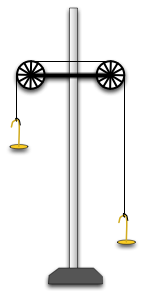
\includegraphics[scale=1.5, angle=0]{lab1.jpg}
\caption{Setup used for this experiment}
\end{figure}

\pagebreak
\section*{Data}
\begin{center}
%\begin{tabular}

%\end{tabular}
\begin{figure}[!ht]
\caption{caption}
\end{figure}
\end{center}

\pagebreak
\section*{Discussion}
\subsection*{Sample Calculations}

\subsection*{Analysis}

\section*{Conclusion}

\end{document}